\documentclass[10pt,conference,draftclsnofoot,onecolumn]{IEEEtran}

\usepackage{graphicx}
\usepackage{amssymb}
\usepackage{amsmath}
\usepackage{amsthm}

\usepackage{alltt}
\usepackage{float}
\usepackage{color}
\usepackage{url}
\usepackage{listings}

\usepackage{balance}
\usepackage[TABBOTCAP, tight]{subfigure}
\usepackage{enumitem}
\usepackage{pstricks, pst-node}

\usepackage{geometry}
\geometry{textheight=8.5in, textwidth=6in}

\newcommand{\cred}[1]{{\color{red}#1}}
\newcommand{\cblue}[1]{{\color{blue}#1}}

\usepackage{hyperref}
\usepackage{geometry}

\def\name{Yi-Jung Chiang}

\hypersetup{
  colorlinks = true,
  urlcolor = black,
  pdfauthor = {\name},
  pdfkeywords = {CS544 "operating systems'' files filesystem I/O},
  pdftitle = {CS 544 Project 2},
  pdfsubject = {CS 544 Project 2},
  pdfpagemode = UseNone
}

\begin{document}

\begin{titlepage}
    \begin{center}
        \vspace*{3.5cm}
        \Large
        \textbf{Project 2}
        \vspace{0.5cm}
        \textbf{Yi-Jung Chiang}
        \vspace{0.8cm}

        CS 544\\
        Spring 2017\\

        \vspace{1cm}

        \textbf{Abstract}\\

        \vspace{0.5cm}
        In this project, I created a SSTF algorithm. After I finished SSTF algorithm, I put this algorithm in my kernel. This idea is similiar to NOOP so I had help looking at its code.  Also, I modified Makefile and Kconfig which are in my kernel.
        \vfill
    \end{center}
\end{titlepage}

\newpage

\begin{figure}
    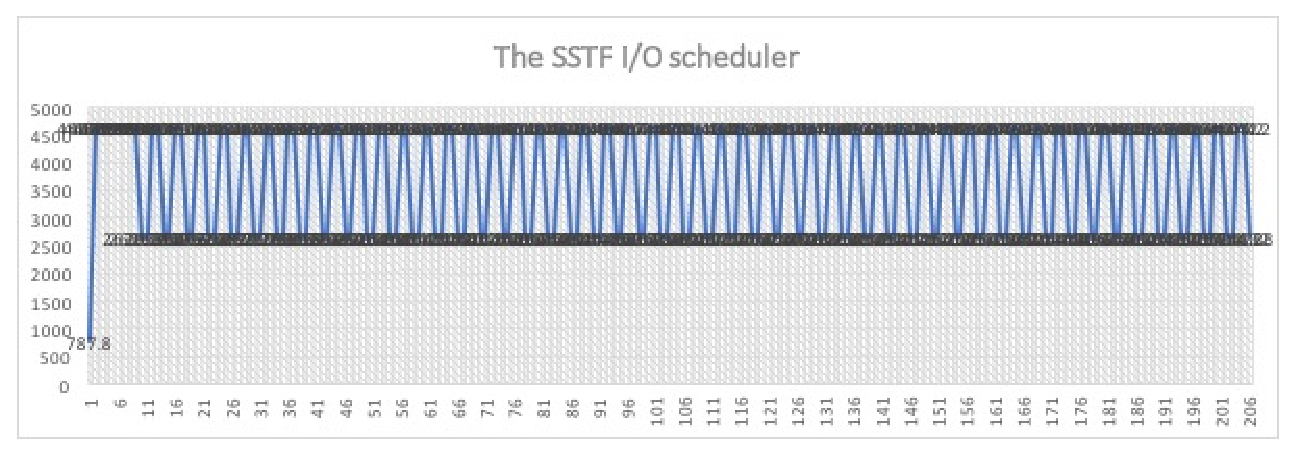
\includegraphics[width=0.8\textwidth]{Picture1.eps}
  \caption{The SSTF I/O scheduler}
  \label{fig:SSTF}
\end{figure}


\section{Concurrency Questions}

\textit{What do you think the main point of this assignment is?}\\

In assignment 2,there are two main points.The first point is how to create SSTF algorithm and use it in my kermnel. The second point is how to use pthread to solve dining philosopher problem. \\

\textit{How did you personally approach the problem? Design decisions, algorithm, etc.}\\

Before I started this assignment, I reviewed the concept of the dining philosophers problem. There are three major solutions I can use to solve this problem. I choose to use there are only four people can eat at the same time. However, although this method can solve deadlock problem, it sill has starvation. About my sstf-iosched.c file, I use old file that exisits in my kernel to modify.  \\



\textit{How did you ensure your solution was correct? Testing details, for instance.}\\

I am sure that my solution was correct through printing many trace statements and values throughout the whole development process. To visually evaluate my solution, I print out at the same time, how many philosophers eat. Also, I print out which forks are used. All results are coreect. \\

\textit{What did you learn?}\\

In this project, I originally only know two solutions which can solve the dining philosopher problem. I also know one more solution which can solve this problem but that solution is super complicated and hard to complete. Also, I learn the concept of SSTF and Noop.  \\





\section{Work Log}
\begin{tabular}{lll} \textbf{Author}
     & \textbf{Date}
     & \textbf{Message}

\\ \hline
Yi-Jung Chiang & 2017-05-02 & Review the dining philosopher problem\\ \hline
Yi-Jung Chiang & 2017-05-02 & Implementing the dining philosopher problem \\ \hline
Yi-Jung Chiang & 2017-05-03 & Finish sstf-iosched.c, makefile and Kconfig.iosched\\ \hline
Yi-Jung Chiang & 2017-05-05 & Upload sstf-iosched.c, makefile and Kconfig.iosched\\ \hline
Yi-Jung Chiang & 2017-05-05 & Implementing look dispatched function \\ \hline
Yi-Jung Chiang & 2017-05-05 & Finish Latex\\ \hline
\end{tabular}



\end{document}